%!TEX program = lualatex

% Name           : WASI_observatory_training.tex
% Author         : Christopher Bennett (chris@east20thst.net)
% Version        : 0.1
% Created on     : 2023-05-16
% Last Edited on : 2023-05-16
% Copyright      : 2023, Christopher Bennett
% License        : This file is in the Public Domain; It may be distributed
%                  and/or modified for any purpose.
% Description    : WASI Observatory training presentation (light).

\documentclass[aspectratio=169, 11pt]{beamer}

% ------ Packages and definitions -----------------------------------------
\usepackage{booktabs} % Better tables
\usepackage{caption} % For sub-figures
\usepackage{subcaption} % For sub-figures
\usepackage[scale=2]{ccicons} % Icons for CC-BY-SA
\usepackage{appendixnumberbeamer} % To use \appendix command
\pdfstringdefDisableCommands{% Fix hyperref translate warning with \appendix
  \def\translate#1{#1}%
}

% ------ Set theme and options --------------------------------------------
\usetheme[background=light,sectionstyle=style4]{trigon2}

% ------ Template graphics ------------------------------------------------
\graphicspath{{images/}}

\titlegraphic{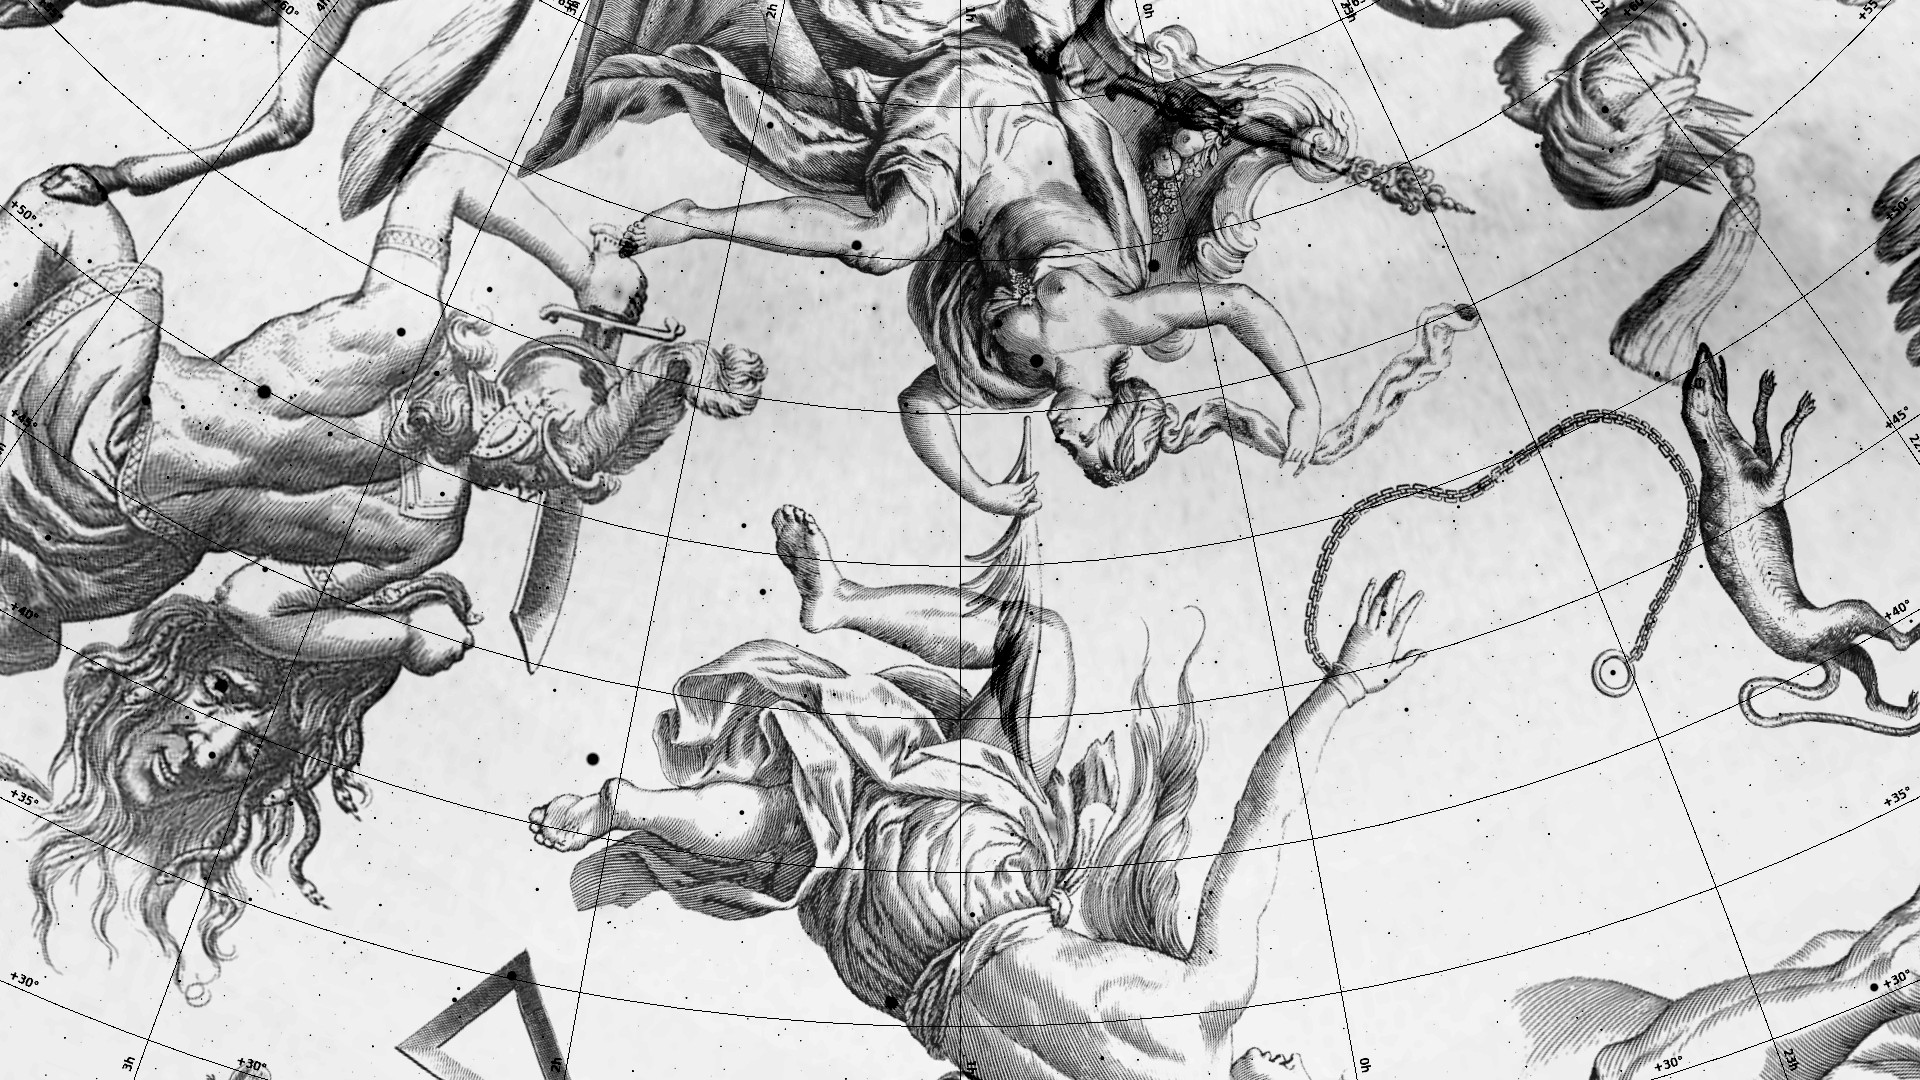
\includegraphics{template/cassiopeia-bg.png}}
\biglogo{template/wasi_full.pdf} % Used on titlepage only
\smalllogo{template/wasi_small.pdf} % Top right corner of regular frames

% ------ Define custom colors ---------------------------------------------
\definecolor{tTheme}{HTML}{800000}  % Red
\definecolor{tPrim}{HTML}{800000}   % Red
\definecolor{tSec}{HTML}{FF0000}    % Light Red
\definecolor{tAccent}{HTML}{808080} % Gray

% ------ Document metadata ------------------------------------------------
\title{Basic Observatory Operations}
% \subtitle{Blaine F. Roelke Memorial Observatory}
\author[JB]{Jeff Burns, Observatory Director}
\institute{Westminster Astronomical Society}
\date{\today}

% -------------------------------------------------------------------------
%                               BEGIN DOCUMENT
% -------------------------------------------------------------------------

\begin{document}

% ------ Create title frame -----------------------------------------------
\titleframe

% ------ Table of contents ------------------------------------------------
\begin{frame}
  \setbeamertemplate{section in toc}[sections numbered]
  \tableofcontents[hideallsubsections]
\end{frame}

%!TEX program = lualatex

% Name           : frames.tex
% Author         : Christopher Bennett (chris@east20thst.net)
% Version        : 0.1
% Created on     : 2023-05-16
% Last Edited on : 2023-05-16
% Copyright      : 2023, Christopher Bennett
% License        : This file is in the Public Domain; It may be distributed
%                  and/or modified for any purpose.
% Description    : WASI Observatory training presentation (frames).

% ==============================================
\section*{Introduction}
% ==============================================

\begin{frame}[t]{Blaine F. Roelke Memorial Observatory}
    \begin{columns}[T]
    \column{0.4\textwidth}
      \centering
      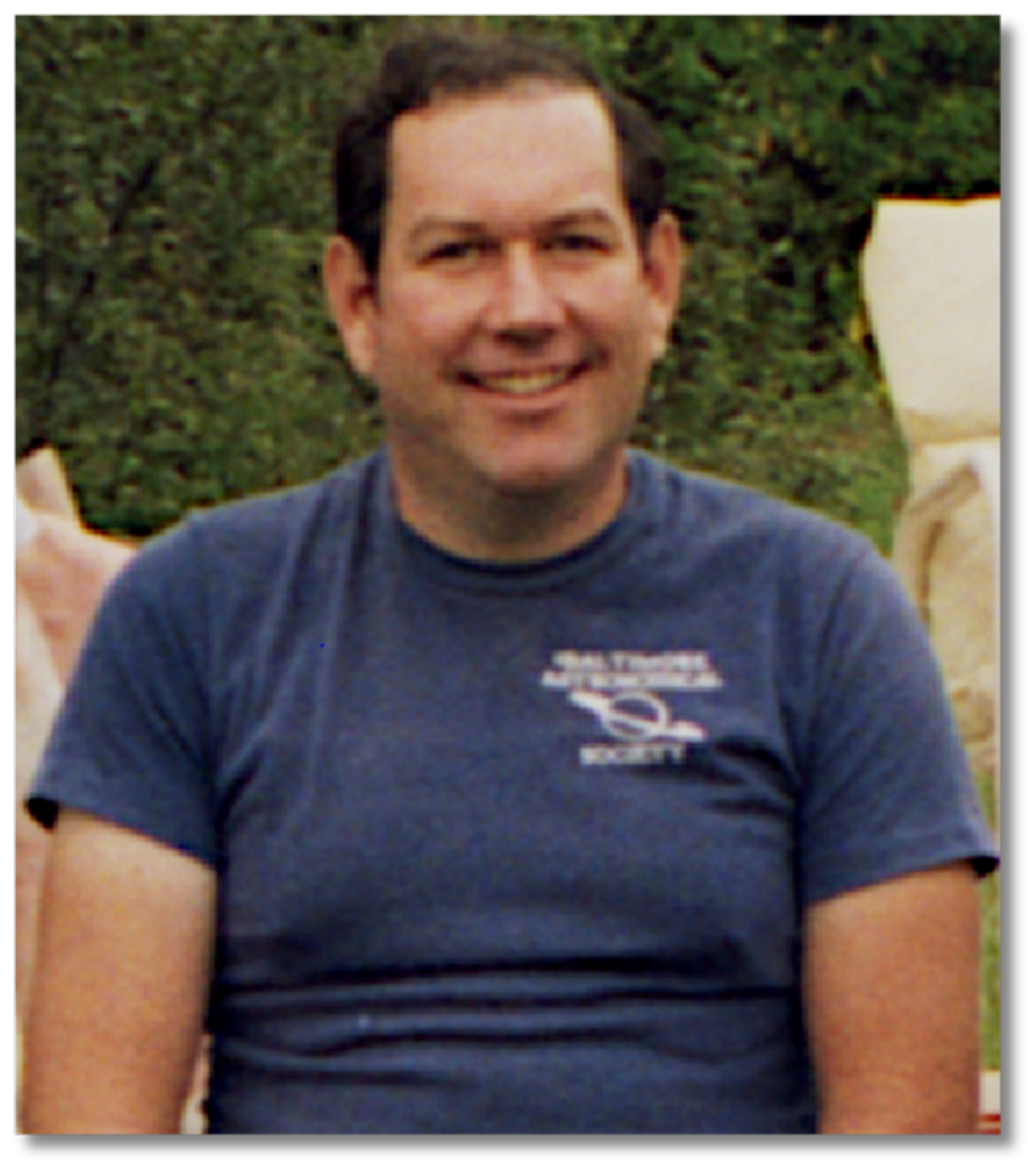
\includegraphics[width=0.8\textwidth]{Blaine_Roelke.pdf}

      \footnotesize Blaine Franklin Roelke (1946-2013) \\
        WASI Charter member since 1984
 
    \column{0.5\textwidth}
      \ \\
      The Blaine F. Roelke Memorial Observatory is home to Westminster
      Astronomical Society's primary instrument, a Celestron 14-inch SCT inside a
      three-meter Ash dome. \\[1ex]
      The telescope and dome were previously owned by Mr.  Roelke and were made
      available to WASI through the generous donation of the Roelke family.
    \end{columns}
\end{frame}


% ==============================================
\section{Astronomy Fundamentals}
% ==============================================

\subsection{Telescopes}
% ==============================================

\begin{frame}{\insertsubsectionhead}
  \centering
    \includegraphicscopyright[height=0.75\textheight]{parts_of_a_telescope.pdf}{
      \href{https://themcdonalds.net/richard/wp/balancing-an-equatorial-mount/}{
      Credit: Richard McDonald, https://themcdonalds.net}}
\end{frame}

%-----------------------------------------------

\begin{frame}{Telescope Types}
  \begin{columns}[T,onlytextwidth]

    \column{0.6\textwidth}
    \centering
      \includegraphicscopyright[height=0.74\textheight]{telescopes.pdf}{
        \href{https://creativecommons.org/licenses/by-sa/4.0/}{
        CC BY-SA 4.0}}

    \column{0.4\textwidth}
      \Large Lenses or Mirrors\\[2ex]
      \begin{itemize}
        \item Refractor
        \item Reflector
        \item Catadioptric
      \end{itemize}

  \end{columns}
\end{frame}

% -----------------------------------------------

\begin{frame}{Aperture \& Focal Length}
  \begin{description}
    \item[Aperture ($d$):] The light grasp of the instrument. (proportional to $d^2$)
    \item[Focal length ($f$):] Determines the scale of the image. ($\arctan{1/f}$)
    \end{description}

  \vfill
  
  \centering
  \includegraphicscopyright[width=0.85\textwidth]{focal_length.pdf}{
    \href{https://creativecommons.org/licenses/by-sa/4.0/}{
    CC BY-SA 4.0}}
\end{frame}

% -----------------------------------------------

\begin{frame}{Focal Ratio}
  \begin{description}
    \item[Focal ratio:] ($f/d$) Determines the apparent brightness of the object. \\
    $f/4$ to $f/6$ is considered ``fast'', $f/10$ to $f/12$ is ``slow''.
    \end{description}
     
  \vfill

  \centering
  \includegraphicscopyright[width=0.85\textwidth]{focal_length.pdf}{
    \href{https://creativecommons.org/licenses/by-sa/4.0/}{
    CC BY-SA 4.0}}
\end{frame}

% -----------------------------------------------

\begin{frame}{Scale \& Magnification}
  \begin{description}
    \item[Image scale:]  ($\arctan{1/f} \times 206265$) The size of the object at the focal plane in arcsec/mm.
    \item[Magnification:] ($f_{\textrm{tel}}/f_{\textrm{eye}}$) The ratio of the telescope focal length to eyepiece focal length.
    \end{description}
     
  \vfill

  \centering
  \includegraphicscopyright[width=0.85\textwidth]{plate_scale.pdf}{
    \href{https://creativecommons.org/licenses/by-sa/4.0/}{
    CC BY-SA 4.0}}
\end{frame}

% -----------------------------------------------

\begin{frame}{Magnification (example)}
  \Large
  \begin{table}[]
    \centering
    \begin{tabular}{@{}lrr@{}}
    \toprule
         & \multicolumn{2}{c}{magnification} \\ \cmidrule(lr){2-3}
    eyepiece & 14in f/11  & 81mm f/6  \\ \midrule
    50mm &   & \\
    30mm &   & \\
    20mm &   & \\ \bottomrule
    \end{tabular}
  \end{table}
  
  \end{frame}
% -----------------------------------------------

\begin{frame}{Magnification}
  \Large
  \begin{table}[]
    \centering
    \begin{tabular}{@{}lrr@{}}
    \toprule
         & \multicolumn{2}{c}{magnification} \\ \cmidrule(lr){2-3}
    eyepiece & 14in f/11  & 81mm f/6  \\ \midrule
    50mm &  $78.2$ &  $9.7$ \\
    30mm & $130.4$ & $16.2$ \\
    20mm & $195.6$ & $24.3$ \\ \bottomrule
    \end{tabular}
  \end{table}
  
  \end{frame}
% -----------------------------------------------

\begin{frame}{Field of View}
  \begin{description}
    \item[Field of view:] The apparent fov of the eyepiece / magnification.
  \end{description}

  \begin{columns}[T,onlytextwidth]
    \column{0.5\textwidth}
    \centering
      \includegraphicscopyright[width=0.68\textwidth]{fov_1.pdf}{
        Credit: Stellarium}

    \column{0.5\textwidth}
    \centering
      \includegraphicscopyright[width=0.68\textwidth]{fov_2.pdf}{}

  \end{columns}
\end{frame}

% -----------------------------------------------

\begin{frame}{Field of View (example)}
  \Large
  \begin{table}[]
    \centering
    \begin{tabular}{lrrr}
    \toprule
         & \multicolumn{3}{c}{field of view} \\ \cmidrule(lr){2-4}
    eyepiece & apparent & 14in f/11  & 81mm f/6  \\ \midrule
    50mm & $60^{\circ}$ &  &  \\
    30mm & $68^{\circ}$ &  &  \\
    20mm & $68^{\circ}$ &  &  \\ \bottomrule
    \end{tabular}
  \end{table}
  
  \end{frame}

% -----------------------------------------------

\begin{frame}{Field of View}
\Large
\begin{table}[]
  \centering
  \begin{tabular}{lrrr}
  \toprule
       & \multicolumn{3}{c}{field of view} \\ \cmidrule(lr){2-4}
  eyepiece & apparent & 14in f/11  & 81mm f/6  \\ \midrule
  50mm & $60^{\circ}$ & $46^{\prime}$ & $6.2^{\circ}$ \\
  30mm & $68^{\circ}$ & $31^{\prime}$ & $4.2^{\circ}$ \\
  20mm & $68^{\circ}$ & $21^{\prime}$ & $2.8^{\circ}$ \\ \bottomrule
  \end{tabular}
\end{table}

\end{frame}

% -----------------------------------------------

\begin{frame}{Altitude-Azimuth Mount}
  \begin{columns}[T,onlytextwidth]

    \column{0.6\textwidth}
    \centering
      \includegraphicscopyright[height=0.74\textheight]{alt-az_mount.pdf}{
        \href{http://themcdonalds.net/classification-of-telescopes/}{
        Credit: Richard McDonald, https://themcdonalds.net}}

    \column{0.4\textwidth}
    \ \\[1ex]
      \Large
      Mounts that move and track along two axes, altitude (up-down) and azimuth (right-left).

  \end{columns}
\end{frame}

% -----------------------------------------------

\begin{frame}{Equatorial Mounts}
  \begin{columns}[T,onlytextwidth]

    \column{0.6\textwidth}
    \centering
      \includegraphicscopyright[height=0.74\textheight]{gem_mount.pdf}{
        \href{http://themcdonalds.net/classification-of-telescopes/}{
        Credit: Richard McDonald, https://themcdonalds.net}}

    \column{0.4\textwidth}
    \ \\[1ex]

      \Large
      Mounts that move along two axes (RA and Dec), but track only in RA. \\[1ex]

      Aligned with the Earth's axis of rotation.

  \end{columns}
\end{frame}


\subsection{Coordinates \& Time}
% ==============================================

\begin{frame}{Horizontal Coordinates}
  \begin{columns}[T,onlytextwidth]

    \column{0.5\textwidth}
    \centering
      \includegraphicscopyright[width=0.9\textwidth]{horizontal.pdf}{
        \href{https://creativecommons.org/licenses/by-sa/4.0/}{
        CC BY-SA 4.0}}

    \column{0.5\textwidth}
    \Large
      \begin{itemize}
        \item Local, Earth-fixed coordinate system.
        \item The fundamental plane is the local horizon.
        \item Azimuth measured in dms clockwise from North.
        \item Altitude measured in dms from the horizon.
      \end{itemize}

  \end{columns}
\end{frame}

% -----------------------------------------------

\begin{frame}{Equatorial Coordinates}
  \begin{columns}[T,onlytextwidth]

    \column{0.5\textwidth}
    \centering
      \includegraphicscopyright[width=0.8\textwidth]{ra_dec.pdf}{
        \href{https://creativecommons.org/licenses/by-sa/4.0/}{
        CC BY-SA 4.0}}

    \column{0.5\textwidth}
    \Large
      \begin{itemize}
        \item The fundamental plane is the equator.
        \item RA measured in hms from the vernal equinox increasing to the East.
        \item Dec measured in dms from the equator, $+90^{\circ}$ at the NCP, and $-90^{\circ}$ at the SCP.
      \end{itemize}

  \end{columns}
\end{frame}

% -----------------------------------------------

\begin{frame}[t]{Time Scales}
  \Large
  \begin{description}
    \item[UTC:] Basis of civil time. Atomic time with a leap second periodically added to keep
     it within 0.9 sec of UT1. (currently 37s.)
    \item[EST:] Local standard time UTC - 5 hours.
    \item[EDT:] Daylight Saving Time (Mar 12-Nov 5) UTC-4.
    \item[JD:] Julian Date, a continuous count of days and fractions since noon Universal Time on January 1, 4713 BC \\
    (January 1, 2000 at 12:00 noon = JD 2451545.0)
  \end{description}
\end{frame}

% -----------------------------------------------

\begin{frame}[t]{Local Sidereal Time (LST)}
  \Large
  \begin{description}
    \item[LST:] Also know as the the Earth Rotation Angle.
    The Right Ascension of the local meridian.\\[1ex]

    Objects with a RA < LST are west of the meridian.\\
    
    Objects with a RA > LST are east of the meridian.
    \end{description}

\end{frame}

% -----------------------------------------------

\begin{frame}{Local Sidereal Time (LST)}
  \begin{columns}[T]
    \column{0.5\textwidth}
      \begin{figure}[ht]
          \begin{subfigure}{0.7\textwidth}
              \frame{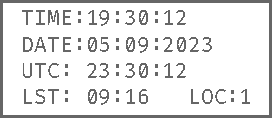
\includegraphics[width=\textwidth]{keypad/AP_menu-time.pdf}}
          \caption{Time/LST}
        \end{subfigure}
        \vspace{\fill}
        \begin{subfigure}{0.7\textwidth}
            \frame{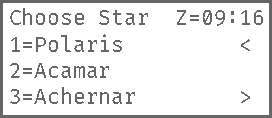
\includegraphics[width=\textwidth]{keypad/AP_menu-objects-5.pdf}}
          \caption{Named Stars}
        \end{subfigure}
      \end{figure}
    \column{0.55\textwidth}
    \ \\[1ex]
    How to find Local Sidereal Time.\\[1.5ex]

    \textbf{Telescope keypad:} From the main menu select \textbf{4=Time/LST} to display the date,
    time and LST.

    The LST is also displayed in the upper right corner of the stars database screen.
  \end{columns}

\end{frame}

% -----------------------------------------------

\begin{frame}{Local Sidereal Time (LST)}
  \begin{columns}[T]
    \column{0.55\textwidth}
    \centering
      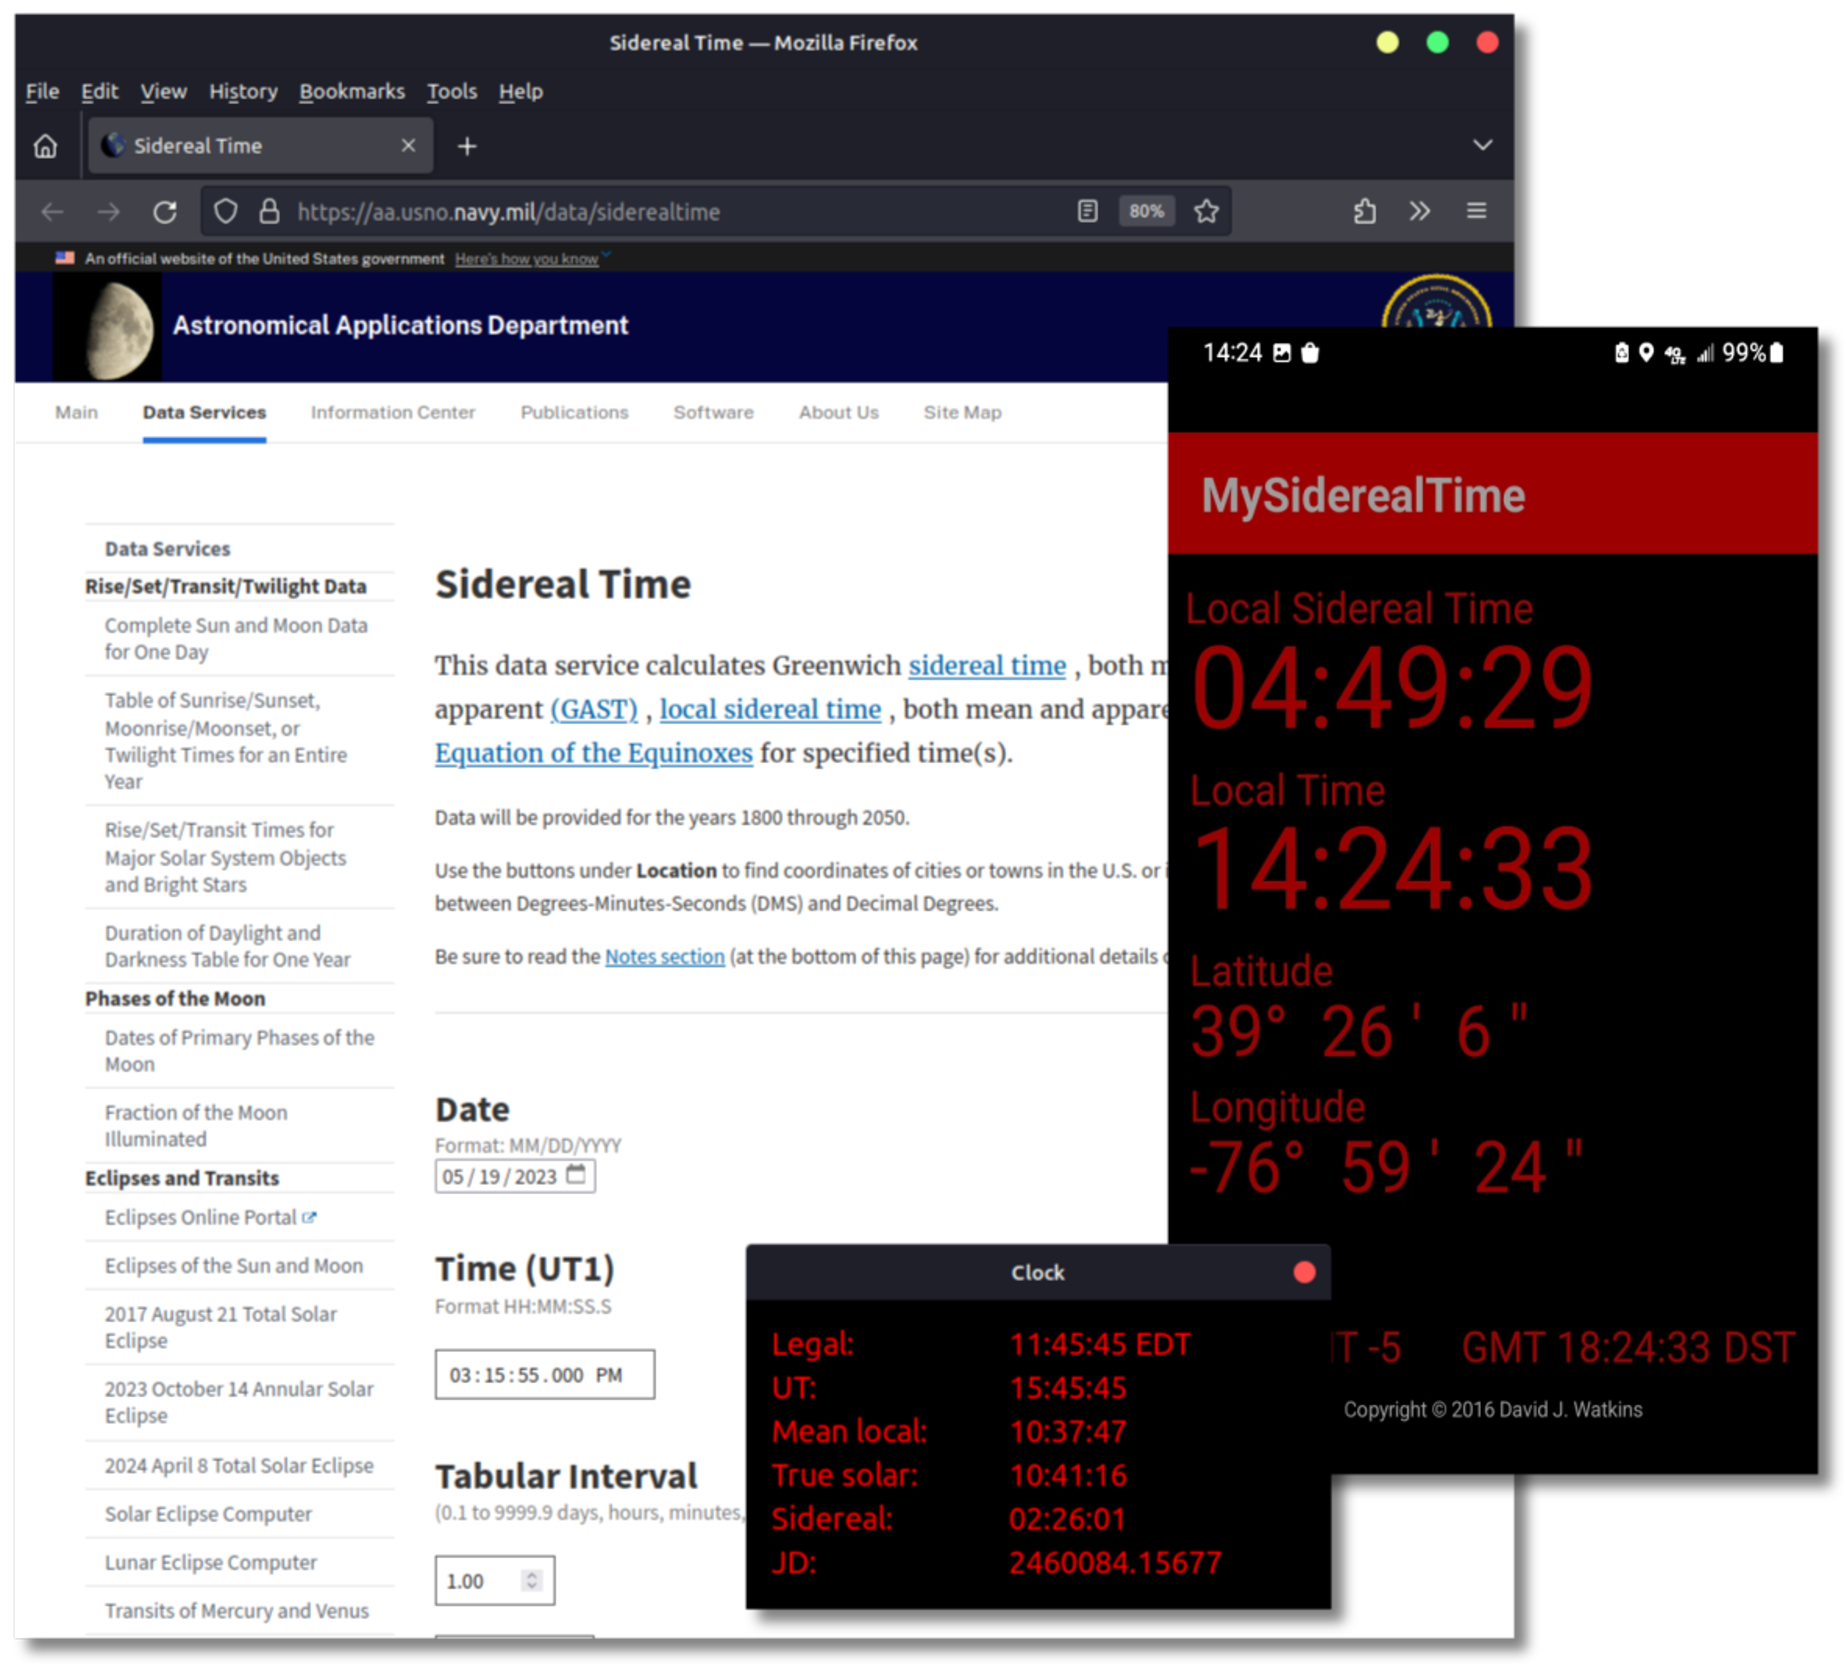
\includegraphics[height=0.8\textheight]{LST_apps.pdf}
    \column{0.45\textwidth}
    \ \\[1ex]

    How to find Local Sidereal Time.\\[1.5ex]

    \textbf{On the internet:} \href{https://aa.usno.navy.mil/data/siderealtime}{USNO Sidereal Time}\\[1.5ex]

    \textbf{Phone apps:} such as \href{https://play.google.com/store/apps/details?id=com.watware.www.mysiderealtime&hl=en}{MySiderealTime}\\[1.5ex]

    \textbf{Software:} such as \href{https://www.ap-i.net/skychart/en/start}{Cartes du Ciel}
  \end{columns}

\end{frame}

\subsection{Constellations \& Asterisms}
% ==============================================

\subsubsection{Constellations}
% ==============================================

\begin{frame}{\insertsubsubsectionhead}
  \centering
  \includegraphicscopyright[width=0.85\textwidth]{allsky.pdf}{
    \href{https://creativecommons.org/licenses/by-sa/4.0/}{
    CC BY-SA 4.0}}
\end{frame}

% -----------------------------------------------

\begin{frame}{\insertsubsubsectionhead}
  \begin{columns}[T,onlytextwidth]

    \column{0.5\textwidth}
    \centering
      \includegraphicscopyright[width=0.8\textwidth]{circumpolar_north.pdf}{
        \href{https://creativecommons.org/licenses/by-sa/4.0/}{
        CC BY-SA 4.0}}

    \column{0.5\textwidth}
    {\Large Circumpolar Constellations}
      \begin{itemize}
        \item Cassiopeia
        \item Cepheus
        \item Draco
        \item Ursa Major
        \item Ursa Minor
        \item Camelopardalis
      \end{itemize}

  \end{columns}
\end{frame}

% -----------------------------------------------

\begin{frame}{\insertsubsubsectionhead}
  \begin{columns}[T,onlytextwidth]

    \column{0.5\textwidth}
    \centering
    \includegraphicscopyright[height=0.76\textheight]{spring_north.pdf}{
      \href{https://creativecommons.org/licenses/by-sa/4.0/}{
      CC BY-SA 4.0}}

    \column{0.5\textwidth}
    {\Large Spring Constellations}
    \begin{columns}[T,onlytextwidth]
      \column{0.5\textwidth}
      \begin{itemize}
        \item Bootes
        \item Canes Venatici
        \item Cancer
        \item Coma Berenices
        \item Leo
        \item Leo Minor
        \item Virgo
        \item Corvus
      \end{itemize}
      \column{0.5\textwidth}
      \begin{itemize}
        \item Crater
        \item Sextans
        \item Hydra
        \item Antlia
        \item Pyxis
        \item Lupus
        \item Centaurus
      \end{itemize}
    \end{columns}
  \end{columns}
\end{frame}

% -----------------------------------------------
\begin{frame}{\insertsubsubsectionhead}
  \begin{columns}[T,onlytextwidth]

    \column{0.5\textwidth}
    \centering
      \includegraphicscopyright[height=0.76\textheight]{summer_north.pdf}{
        \href{https://creativecommons.org/licenses/by-sa/4.0/}{
        CC BY-SA 4.0}}

    \column{0.5\textwidth}
    {\Large Summer Constellations}
    \begin{columns}[T,onlytextwidth]
      \column{0.5\textwidth}
      \begin{itemize}
        \item Cygnus
        \item Lyra
        \item Corona Borealis
        \item Vulpecula
        \item Delphinus
        \item Sagitta
        \item Hercules
        \item Serpens
      \end{itemize}
      \column{0.5\textwidth}
      \begin{itemize}
        \item Ophiuchus
        \item Equuleus
        \item Aquila
        \item Capricornus
        \item Scutum
        \item Libra
        \item Sagittarius
        \item Scorpius
      \end{itemize}
    \end{columns}
  \end{columns}
\end{frame}

% -----------------------------------------------

\begin{frame}{\insertsubsubsectionhead}
  \begin{columns}[T,onlytextwidth]

    \column{0.5\textwidth}
    \centering
    \includegraphicscopyright[height=0.76\textheight]{fall_north.pdf}{
      \href{https://creativecommons.org/licenses/by-sa/4.0/}{
      CC BY-SA 4.0}}

    \column{0.5\textwidth}
    {\Large Fall Constellations}
    \begin{columns}[T,onlytextwidth]
      \column{0.5\textwidth}
      \begin{itemize}
        \item Perseus
        \item Triangulum
        \item Andromeda
        \item Lacerta
        \item Aries
        \item Pegasus
      \end{itemize}
      \column{0.5\textwidth}
      \begin{itemize}
        \item Pisces
        \item Cetus
        \item Aquarius
        \item Sculptor
        \item Pisces Austrinus
        \item Grus
      \end{itemize}
    \end{columns}
  \end{columns}
\end{frame}

% -----------------------------------------------

\begin{frame}{\insertsubsubsectionhead}
  \begin{columns}[T,onlytextwidth]

    \column{0.5\textwidth}
    \centering
    \includegraphicscopyright[height=0.76\textheight]{winter_north.pdf}{
      \href{https://creativecommons.org/licenses/by-sa/4.0/}{
      CC BY-SA 4.0}}

    \column{0.5\textwidth}
    {\Large Winter Constellations}
    \begin{columns}[T,onlytextwidth]
      \column{0.5\textwidth}
      \begin{itemize}
        \item Auriga
        \item Gemini
        \item Taurus
        \item Orion
        \item Canis Minor
        \item Canis Major
        \item Monoceros
      \end{itemize}
      \column{0.5\textwidth}
      \begin{itemize}
        \item Eridanus
        \item Lepus
        \item Puppis
        \item Columba
        \item Caelum
        \item Fornax
      \end{itemize}
    \end{columns}
  \end{columns}
\end{frame}

\subsubsection{Asterisms}
% ==============================================

\begin{frame}{\insertsubsubsectionhead}
  \begin{columns}[T,onlytextwidth]

    \column{0.5\textwidth}
    \centering
      \includegraphicscopyright[width=0.8\textwidth]{dipper.pdf}{
        \href{https://creativecommons.org/licenses/by-sa/4.0/}{
        CC BY-SA 4.0}}

    \column{0.5\textwidth}
    \ \\
    \Large Big Dipper: \\[1ex]

    Dubhe ($\alpha$ UMa) and Merak ($\beta$ UMa) are the pointer stars for Polaris.
    
    
  \end{columns}
\end{frame}
% -----------------------------------------------

\begin{frame}{\insertsubsubsectionhead}
  \begin{columns}[T,onlytextwidth]

    \column{0.5\textwidth}
    \centering
    \includegraphicscopyright[width=0.8\textwidth]{summer_triangle.pdf}{
      \href{https://creativecommons.org/licenses/by-sa/4.0/}{
      CC BY-SA 4.0}}

    \column{0.5\textwidth}
    \ \\
    \Large Summer Triangle: \\[1ex]
    \large
    Deneb ($\alpha$ Cyg)\\
    Altair ($\alpha$ Aqu)\\
    Vega ($\alpha$ Lyr)\\
    The most prominent asterism in the Summer sky.
    
  \end{columns}
\end{frame}

% -----------------------------------------------

\begin{frame}{\insertsubsubsectionhead}
  \begin{columns}[T,onlytextwidth]

    \column{0.5\textwidth}
    \centering
    \includegraphicscopyright[width=0.8\textwidth]{winter_hexagon.pdf}{
      \href{https://creativecommons.org/licenses/by-sa/4.0/}{
      CC BY-SA 4.0}}

    \column{0.5\textwidth}
    \ \\
    \Large Winter Hexagon \\[1ex]
    \large
     Pollux ($\beta$ Gem )\\
     Capella ($\alpha$ Ar)\\
     Aldebaran ($\alpha$ Tau)\\
     Rigel ($\beta$ Ori)\\
     Sirius ($\alpha$ CMa)\\
     Procyon ($\alpha$ CMn).\\
    Many of the best objects of the winter sky.
    
  \end{columns}
\end{frame}

% -----------------------------------------------

\begin{frame}{\insertsubsubsectionhead}
  \begin{columns}[T,onlytextwidth]

    \column{0.5\textwidth}
    \centering
    \includegraphicscopyright[width=0.8\textwidth]{spring_triangle.pdf}{
      \href{https://creativecommons.org/licenses/by-sa/4.0/}{
      CC BY-SA 4.0}}

    \column{0.5\textwidth}
    \ \\
    \Large Spring Triangle \\[1ex]
    \large
    Arcturus ($\alpha$ Boo)\\
    Spica ($\alpha$ Vir)\\
    Denebola ($\beta$ Leo).\\
    Rich galaxy hunting ground.
    
  \end{columns}
\end{frame}

% -----------------------------------------------

\begin{frame}{\insertsubsubsectionhead}
  \begin{columns}[T,onlytextwidth]

    \column{0.5\textwidth}
    \centering
    \includegraphicscopyright[width=0.8\textwidth]{pegasus_square.pdf}{
      \href{https://creativecommons.org/licenses/by-sa/4.0/}{
      CC BY-SA 4.0}}

    \column{0.5\textwidth}
    \ \\
    \Large The Pegasus Square \\[1ex]
    \large
     Markab ($\alpha$ Peg)\\
     Scheat ($\beta$ Peg)\\
     Algenib ($\gamma$ Peg)\\
     Alpheratz ($\alpha$ And)
    
  \end{columns}
\end{frame}

\subsection{Star Catalogs}
% ==============================================

\subsubsection{Catalogs \& Star Charts}
% ==============================================
\begin{frame}{The Names of Stars}
  \Large
  \begin{itemize}
    \item Named Stars. \\
    There are 451 \href{https://www.iau.org/public/themes/naming_stars/}{IAU named stars}.
    The keypad database has 200.
    \item Bayer Designation (e.g. $\alpha$ Orionis).\\
    From the \emph{Uranometria} of Johann Bayer. The brightest stars in each constellation are labeled with
    lowercase Greek letters.
    \item Flamsteed Designation (e.g. 61 Cygni).\\
    From the \emph{Atlas Coelestis} of John Flamsteed. A number and constellation designating most of the
    naked eye stars in the sky.
  \end{itemize}
\end{frame}

% -----------------------------------------------

\begin{frame}{\insertsubsubsectionhead}
  \Large
  Strasbourg Astronomical Data Center \href{https://cds.unistra.fr/}{(https://cds.unistra.fr)}.
  \begin{itemize}
    \item Bonner Durchmusterung (BD +7 1055)
    \item Henry Draper Catalogue (HD 39801)
    \item Yale Bright Star Catalogue (HR 2061)
    \item Smithsonian Astrophysical Observatory Catalogue (SAO 113271)
    \item Positions and Proper Motions Catalogue (PPM 149643)
  \end{itemize}
\end{frame}

% -----------------------------------------------

\begin{frame}{\insertsubsubsectionhead}
  \Large
  \begin{itemize}
    \item Variable Stars (e.g. RR Lyrae)\\
    Designated by one or two letters R-Z and the constellation, then subsequently
    by numeric designation (e.g. V1500 Cygni))
    \item Double Stars (e.g. $\alpha$ UMi Aa, Ab, B).\\
    The components of multiple star systems are labeled with upper and lower case letters.
    You will also find multiple stars in the Aitken Double Star catalog (ADS 1477 Aa) and
    the Washington Double Star catalog (WDS J02318+8916 Aa).
  \end{itemize}
\end{frame}

% -----------------------------------------------

\begin{frame}{\insertsubsubsectionhead}
  \Large
  Modern large scale surveys:
  \begin{itemize}
    \item Tycho-2: Positions, proper motions, and magnitudes for 2,539,913
    of the brightest stars (TYC 3521-1800-1).
    \item USNO CCD Astrograph Catalog (UCAC): Positions and magnitudes for 113 million
    stars 8 to 16 magnitude. (UCAC4 712-056369)
    \item Gaia: positions and magnitudes for 1.7 billion stars, including distances
    and proper motions for more than 1.3 billion stars \\(DR2 1415230383033121024).
  \end{itemize}
\end{frame}

\subsubsection{Deep Sky Objects}
% ==============================================

\begin{frame}{\insertsubsubsectionhead}
  \Large
  Strasbourg Astronomical Data Center \href{https://cds.unistra.fr/}{(https://cds.unistra.fr)}.
  \begin{itemize}
    \item New General Catalogue (NGC/IC): 7,840/5,386 objects.
    \item Lynds Bright Nebulae (LBN): 1,125 bright diffuse nebulae.
    \item Lynds Dark Nebulae (LDN): 1,791 dark molecular clouds.
    \item Uppsala Galaxy Catalog (UGC): 12,940 nearby galaxies in the northern sky.
  \end{itemize}
  \hspace{1em} many more \dots
\end{frame}

% -----------------------------------------------

\begin{frame}{Observing Lists}
  \Large
  Astronomical League \href{https://www.astroleague.org/al/obsclubs/AlphabeticObservingClubs.html}{(https://www.astroleague.org)}.

  \begin{itemize}
    \item Messier: 110 deep sky objects cataloged by Charles Messier.
    \item Caldwell: 109 additional bright deep sky objects compiled by Sir Patrick Moore.
    \item Herschel 400: 400 of the best deep sky objects from the NGC cataloged by William Herschel.
  \end{itemize}
  \hspace{1em} many more \dots
\end{frame}

\subsubsection{The Solar System}
% ==============================================

\begin{frame}{\insertsubsubsectionhead}
  \framesubtitle{JPL Solar System Dynamics \href{https://ssd.jpl.nasa.gov/}{(https://ssd.jpl.nasa.gov)}.}
  
  {\Large Provides orbits, physical characteristics, and discovery circumstances
  for most known natural bodies in our solar system.} \\[1ex]

  \begin{itemize}
  \item \textbf{Horizons:} ephemeris for 1,283,931 asteroids, 3,875 comets, 290 planetary satellites.
  \item \textbf{Small-Body Database:} orbital elements, physical parameters, etc.
  \item \textbf{Small-Body Identification:} all known small bodies a region at a specified time time.
  \item \textbf{Small-Body Observability:} all small bodies observable from a specified location.
  \item \textbf{Orbit Viewer:} display the orbits of the planets, their satellites, and small bodies.
  \end{itemize}

\end{frame}

% -----------------------------------------------

\begin{frame}{\insertsubsubsectionhead}
  \framesubtitle{IAU Minor Planet Center \href{https://www.minorplanetcenter.net/}{(https://www.minorplanetcenter.net)}.}
  
  {\Large The Minor Planet Center (MPC) is the worldwide location for receipt and distribution
  of positional data of minor planets, comets and satellites of the major planets.}\\[1ex]

  \begin{itemize}
  \item Ephemeris Service
  \item Orbital elements (MPCORB)
  \item Observation Planning and target lists
  \item Observing guides
  \end{itemize}

\end{frame}


% ==============================================
\section{The Blaine F. Roelke Observatory}
% ==============================================

\subsection{Facility \& Dome}
% ==============================================

\begin{frame}[t]{\insertsubsectionhead}
  \Large
  \begin{itemize}
    \item 3-meter diameter Ash dome.
    \item Equipped with AC electrical service.
    \item White and red lighting inside and out.
    \item Internet access through the BBNC network.
  \end{itemize}
\end{frame}

\subsection{Telescopes}
% ==============================================

\begin{frame}[t]{Celestron C14}
  \Large
  \begin{itemize}
    \item 14-inch (356mm) Schmidt-Cassegrain.
    \item Focal ratio of f/11.
    \item Primary mirror focus as well as a dual speed Crayford focuser.
    \item Suffers from ``mirror flop'' especially after a meridian flip.\\
          (Causes alignment change, slight focus change.)
  \end{itemize}
 \end{frame}

% -----------------------------------------------

\begin{frame}[t]{William Optics 81mm APO}
  \Large
  \begin{itemize}
    \item 81 mm, APO triplet.
    \item Focal ratio of f/6.
    \item Wide field of view for large objects: Moon, open star clusters, etc.
  \end{itemize}

\end{frame}

% -----------------------------------------------

% \begin{frame}{Lunt 50mm H-Alpha}

% \end{frame}

% -----------------------------------------------

\begin{frame}{AP 1100GTO GEM Mount}
  \begin{columns}[T,onlytextwidth]
    \column{0.5\textwidth}
      The Astro-physics 1100GTO German Equatorial Mount is a high performance
      computer controlled observatory mount.\\[2ex]

      \begin{itemize}
        \item High capacity payload (110 lb)
        \item Precision DC servo motor and gearbox 
        \item GTOCP4 control box and keypad
        \item Astro-Physics Command Center (APCC)
        \item Quick and easy setup and operation
      \end{itemize}

    \column{0.5\textwidth}
      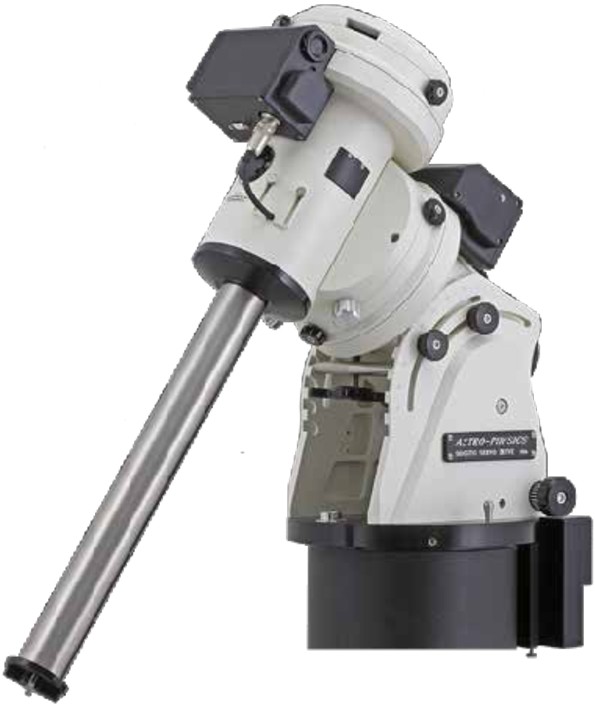
\includegraphics[width=\textwidth]{1100gto-cp4.pdf}

  \end{columns}
\end{frame}


% ==============================================
\section{Scheduling \& Access}
% ==============================================

\begin{frame}{Basic Rules for Use}
  \Large
  \begin{itemize}
    \item Follow proper sign-up procedures.
    \item Leave everything better than you found it.
    \item Food and drinks are fine. Take all trash with you when you leave.
    \item No smoking in and around the observatory.
    \item No alcohol on BBNC grounds. Follow all BBNC rules.
    \item Only perform operations that you are trained and qualified for.
    \item Please come to the club work-sessions.
    \item Occasionally volunteer for public nights.
    \item Damage that isn't usual ``wear and tear'' must be replaced.
  \end{itemize}
\end{frame}

% -----------------------------------------------

\begin{frame}{Operator Qualification}
  \Large
  Two classes of operators:
  \begin{description}
    \item[Basic:] Startup and initialize the telescope, perform basic telescope operations.
     Make no changes to the configuration of the telescope and mount.
    \item[Advanced:] Can align/realign the telescope, make changes to the configuration that require
     re-balancing the telescope. \\[1ex]
     Adjust polar alignment and collimation (with permission of the observatory director).
  \end{description}
\end{frame}

% -----------------------------------------------

\begin{frame}{Operator Qualification}
  \Large
  You must take the class for basic operation (today's class!)
  \begin{itemize}
    \item Demonstration of observatory operation (4 trainees at a time)
    \item Individual practical test of your ability to operate the dome and telescope.
     (you can use your notes, manuals, etc.)
    \item If possible trainees should operate the observatory with another experienced
      member once before operating alone.
    \item Advanced operators must demonstrate their skills after a significant number of observing sessions
  \end{itemize}
\end{frame}

% -----------------------------------------------

\begin{frame}{Scheduling}
  \Large
  Advance sign-up is required for observatory use.
  \begin{itemize}
    \item The observatory director (OD) and BBNC must be notified at least 24 hours prior
    to use (the OD will contact BBNC for you).
    \item You must have confirmation before use. (no answer isn't an OK!)
  \end{itemize}

  Procedure:
  \begin{itemize}
    \item Call or email Jeff Burns at 240-459-5100 or jeff.burns@areva.com.
    \item Specify the night and a back-up weather date if you have one.
    \item The OD will contact BBNC and reply with a confirmation.
  \end{itemize}
\end{frame}

% -----------------------------------------------

\begin{frame}{Availability}
  \Large
  The observatory has been under-utilized, especially given the closure due to COVID.
  \begin{itemize}
    \item It is still rare that there is a conflict between uses.
    \item Use by the outdoor school will have priority during the week.
    \item Regularly scheduled public events, whether by BBNC or WASI will have priority.
    \item Other priorities are listed in the observatory policy document
  \end{itemize}
\end{frame}

% -----------------------------------------------

\begin{frame}{Access}
  \Large
  When you have completed training:
  \begin{itemize}
    \item The OD will give you a key code for the lock.
    \item Do not share your code with anyone.
    \item Codes will occasionally be changed.\\
      (check with the OD if you have not used it in a while).
    \item Users will also get the code to the key box for the accessory cases (eyepieces, cameras, etc.)
    \item The top case is for BBNC and Outdoor SChool staff, the bottom holds WASI equipment.
  \end{itemize}
\end{frame}


% ==============================================
\section{Opening \& Closing}
% ==============================================

\subsection{Opening The Observatory}
%==============================================
\begin{frame}{\insertsubsectionhead}
  \Large
  \begin{itemize}
    \item Enter your four digit code into the lock-set.
    \item Open the door, go in. (Use caution going in/out, low clearance!)
    \item Turn on the outside red light and leave it on while the observatory
       is in use.
    \item Turn on the inside white and red lights as required. Please use all
       inside lights until you are well oriented.\\
       (Light switches are on the left inside the door)
  \end{itemize}
\end{frame}

% -----------------------------------------------
\begin{frame}{\insertsubsectionhead}
  \Large
  \begin{itemize}
    \item Inspect the facilities for any evidence of vandalism, theft,
     or weather damage. \\
     (For major issues please call the OD or BBNC staff ASAP.)
    \item Check the log for any issues during previous sessions.\\
     (In the 3-ring binder on the desk.)
    \item Start a new log to record your activities. \\
     (Note any discrepancies in your inspection.)
    \item A complete checklist and contact information are in the binder.
  \end{itemize}
\end{frame}

% -----------------------------------------------

\begin{frame}[t]{Observatory Log}
\begin{columns}[T]
  \column{0.45\textwidth}
    \begin{figure}[h]
        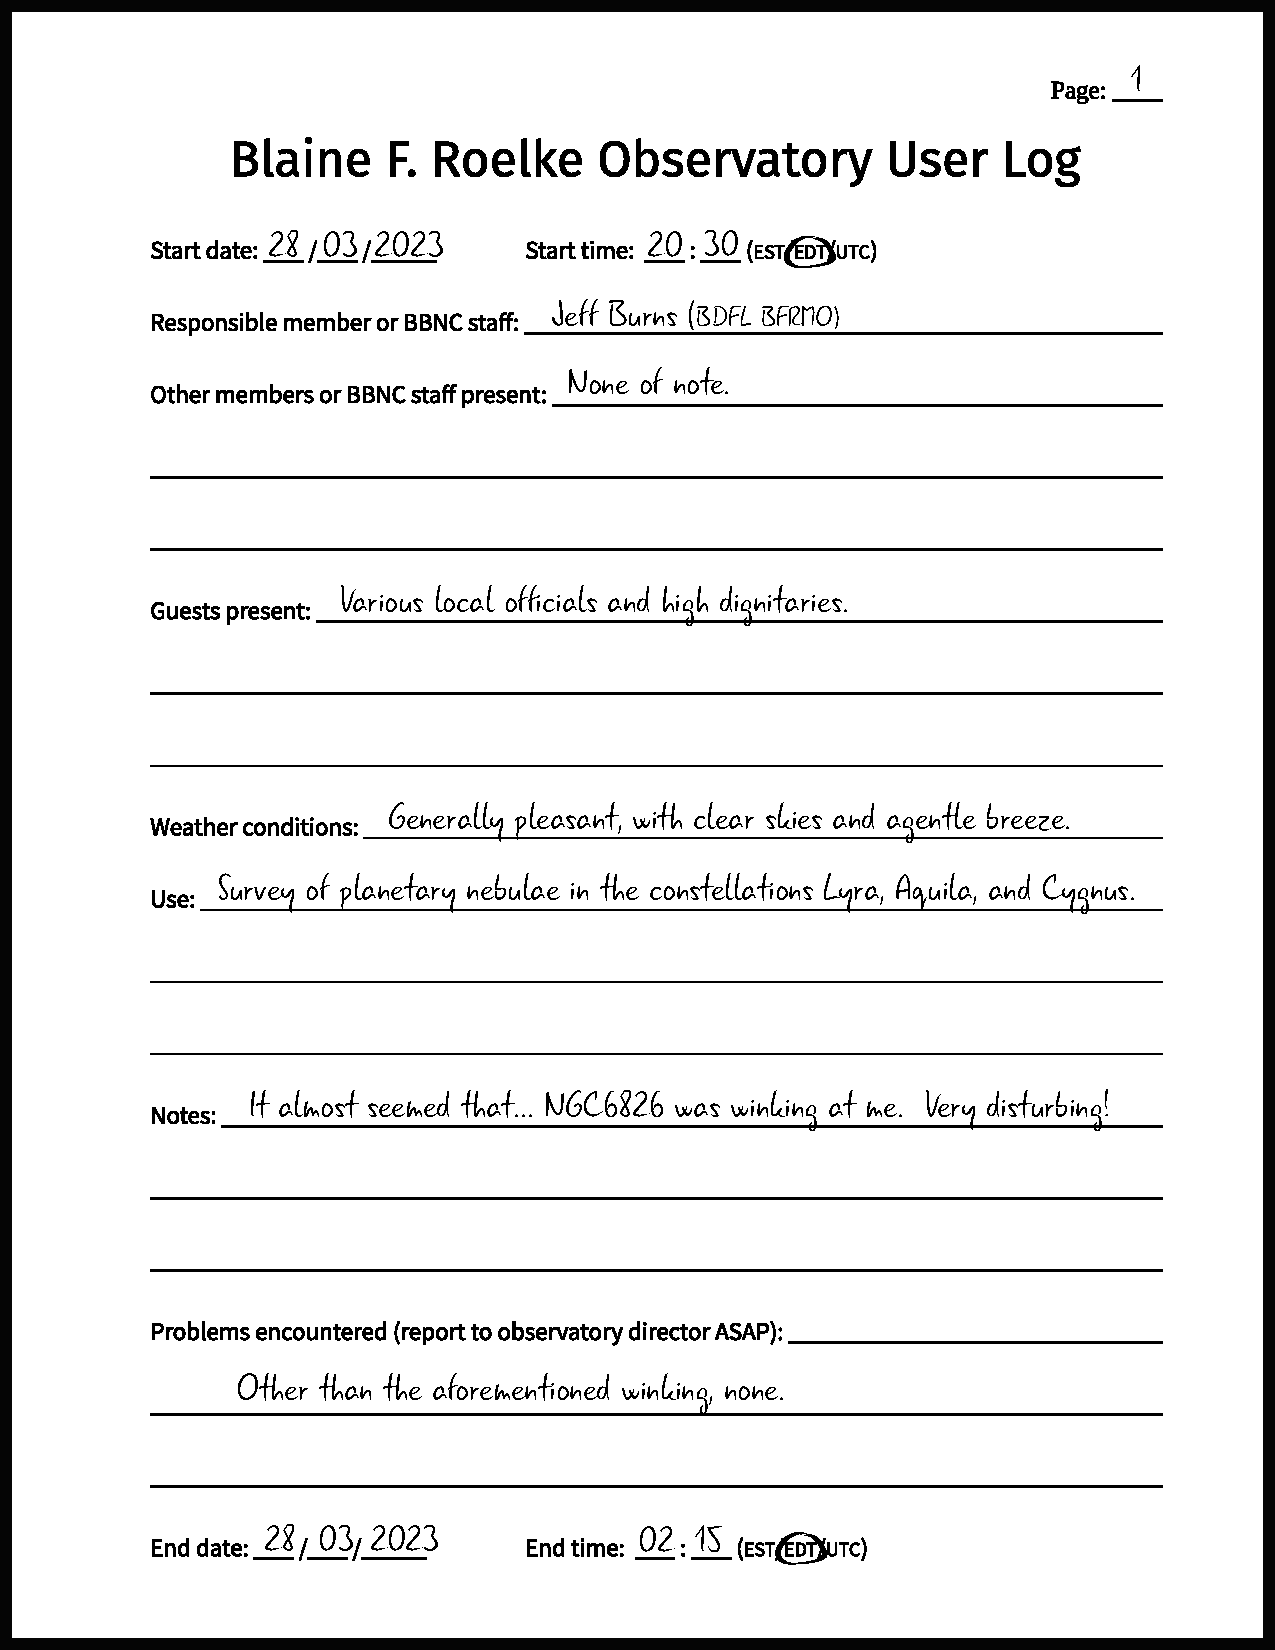
\includegraphics[height=0.7\textheight]{observatory_log.pdf}
      \caption{observatory log}
    \end{figure}
  \column{0.55\textwidth}

  {\Large
    The Observatory log should include:}
    \begin{itemize}
      \item The date and time.
      \item The primary user's name plus other members or staff present.
      \item Any guests present.
      \item Weather conditions.
      \item The purpose of your observations and any notes that might be of interest.
      \item Any problems encountered.\\
            (Report major problems to the OD.)
    \end{itemize}
\end{columns}
\end{frame}


\subsection{Dome Operation}
%==============================================

\begin{frame}[t]{\insertsubsectionhead}
  \begin{columns}[T]
    \column{0.45\textwidth}
    \centering
    \includegraphicscopyright[height=0.75\textheight]{dome_operation.pdf}{
      \href{https://creativecommons.org/licenses/by-sa/4.0/}{
      CC BY-SA 4.0}}
    \column{0.55\textwidth}
  
    \large
      \begin{itemize}
        \item Hook the eyelet with cordless drill/hook. 
        \item Run the drill counterclockwise on medium speed until open.
        \item If observing near zenith, pull the release chain while starting to open.
        \item if observing near the horizon leave the lower section attached.
        \item Rotate the dome as required using rope tied to handles
      \end{itemize}
  \end{columns}
  \end{frame}

\subsection{Startup and Initialization}
%==============================================

\begin{frame}[t]{\insertsubsectionhead}
  \begin{columns}[T]
    \column{0.5\textwidth}
    \centering
    \includegraphicscopyright[height=0.75\textheight]{C14_telescope.pdf}{
      \href{https://creativecommons.org/licenses/by-sa/4.0/}{
      CC BY-SA 4.0}}
    \column{0.5\textwidth}
      \Large
      \begin{itemize}
        \item Uncover the telescope.
        \item Remove aperture covers.
        \item Rotate the finder and diagonal to a convenient position.
        \item Install a low power eyepiece in each telescope.
      \end{itemize}
  \end{columns}
  \end{frame}

% -----------------------------------------------

\begin{frame}[t]{\insertsubsectionhead}
    The mount should be balanced, aligned and left in park position 3. All you
    need to do is connect power, the system will initialize and the Main Menu
    will appear on the keypad. You can go directly to the Objects Menu and
    enter the desired objects to be viewed.
  \begin{columns}[T]
    \column{0.55\textwidth}
      \begin{figure}[h]
          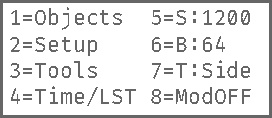
\includegraphics[width=0.8\textwidth]{keypad/AP_menu-1.pdf}
        \caption{main menu}
      \end{figure}
    \column{0.45\textwidth}
      \begin{itemize}
          \item[] \textbf{1=Objects} (objects menu)
          \item[] \textbf{4=Time/LST} (verify date and time)
          \item[] \textbf{5=S:900}   (slew rate)
          \item[] \textbf{6=b:200}   (button rate)
          \item[] \textbf{7=T:Side}  (tracking rate)
      \end{itemize}
  \end{columns}
\end{frame}

% -----------------------------------------------
\begin{frame}[t]{\insertsubsectionhead}
    \begin{columns}[T]
    \column{0.55\textwidth}
      \begin{figure}[h]
          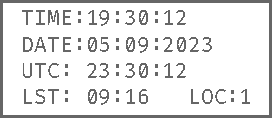
\includegraphics[width=0.8\textwidth]{keypad/AP_menu-time.pdf}
        \caption{Time/LST}
      \end{figure}
    \column{0.45\textwidth}
    \ \\[0.25ex]
    Press \textbf{4=Time/LST} to verify the time.\\[1ex]

    Date, time, and local sidereal time (LST) should match. The time should be
    accurate within a minute or two to ensure accurate pointing and tracking.\\[1ex]

    Press hold \textbf{MENU} to return to the main menu.
  \end{columns}
\end{frame}

% -----------------------------------------------
\begin{frame}[t]{\insertsubsectionhead}
    \begin{columns}[T]
    \column{0.52\textwidth}
    \begin{figure}[ht]
      \begin{subfigure}{0.67\textwidth}
          \frame{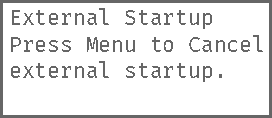
\includegraphics[width=\textwidth]{keypad/AP_menu-init-ext.pdf}}
      \caption{external startup}
    \end{subfigure}
    \vspace{\fill}
    \begin{subfigure}{0.67\textwidth}
        \frame{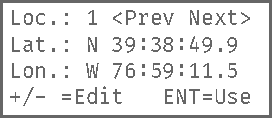
\includegraphics[width=\textwidth]{keypad/AP_menu-init-loc.pdf}}
      \caption{location}
    \end{subfigure}
  \end{figure}
    \column{0.45\textwidth}
    \ \\[0.25ex]
    If the mount was not properly shut down during the previous observing
    session you may see the External Startup or Location Selections screen.\\[1ex]

    Press \textbf{Menu} to cancel External Startup\\[1ex]

    On the Location screen press \textbf{ENT} to use loc 1.
    (there should only be one location)

  \end{columns}
\end{frame}

% -----------------------------------------------
\begin{frame}[t]{\insertsubsectionhead}
    \begin{columns}[T]
    \column{0.55\textwidth}

      \begin{figure}[ht]
          \begin{subfigure}{0.67\textwidth}
              \frame{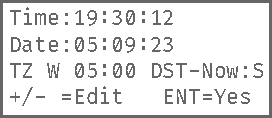
\includegraphics[width=\textwidth]{keypad/AP_menu-init-time.pdf}}
          \caption{time}
        \end{subfigure}
        \vspace{\fill}
        \begin{subfigure}{0.67\textwidth}
            \frame{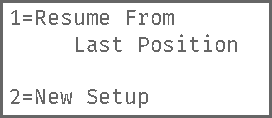
\includegraphics[width=\textwidth]{keypad/AP_menu-init-resume.pdf}}
          \caption{resume}
        \end{subfigure}
      \end{figure}
    \column{0.45\textwidth}
    \ \\[0.25ex]
    Verify that the time and date are correct.\\[1ex]

    Press \textbf{ENT} to accept or \textbf{+/-} to edit the date and
    time.\\[1ex]

    Press \textbf{1} to resume from last position.\\[1ex]

    From the main menu select \textbf{1=Setup} then \textbf{4=Kpd, Mnt, Park},
    and \textbf{7=Auto-connect:YES} to return it to the default setup.

  \end{columns}
\end{frame}


\subsection{Shutdown Procedures}
% ==============================================

\begin{frame}[t]{\insertsubsectionhead}
  \begin{columns}[T]
    \column{0.45\textwidth}
      \centering
      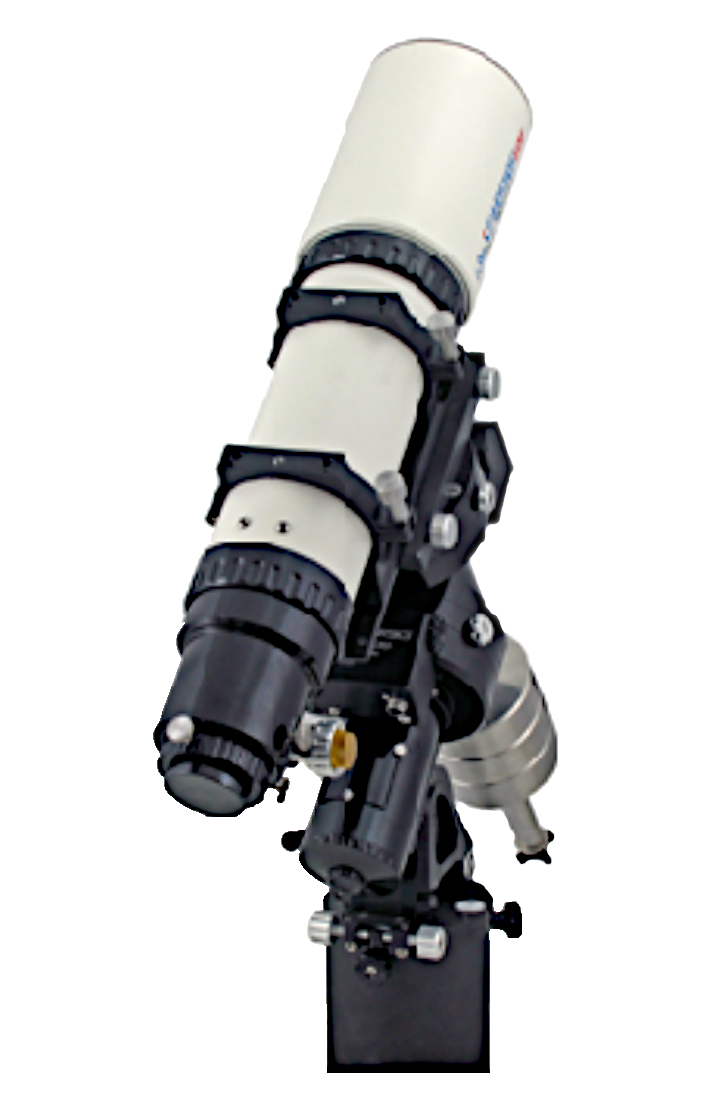
\includegraphics[height=0.8\textheight]{p3.png}
    \column{0.55\textwidth}
    Go to the quick-access menu [\textbf{+/-}] select \textbf{4=Kpd, Mnt,
    Park} and park position 3.\\[1ex]

    Turn off the power, lower the pier, replace all covers.

  \end{columns}
\end{frame}

\subsection{Closing the Observatory}
% ==============================================
\begin{frame}{\insertsubsectionhead}
  \Large
  \begin{itemize}
    \item Turn the dome so the slit is roughly southeast.
    \item Use the drill/hook to close the dome slit (clockwise rotation).
    \item Power off other electrical equipment.
    \item Put away all accessories, lock up accessory cases.
    \item Look around, leave things in better shape than you found them.
    \item Make sure log sheet is complete.
    \item Turn off lights (including external red light).
    \item Exit observatory making sure door is locked behind you.
  \end{itemize}
 \end{frame}

\subsection{Emergencies and Severe Weather}
% ==============================================
\begin{frame}[t]{Emergency Contacts}
  
  {\LARGE\centering
  \textcolor{red}{For police, fire, or medical emergencies: Dial 911}}

  For problems related to the nature center buildings or grounds:

  \textbf{Dawn Harry} (Park Superintendent)\\
  (443) 340-0943

  For problems related to the observatory or equipment:

  \textbf{Jeff Burns} (Observatory Director)\\
  (240) 459-5100, Jeff.burns@areva.com

  \textbf{Curt Roelle}\\
  (443) 340-7895, roelle1@yahoo.com 
\end{frame}

% -----------------------------------------------

\begin{frame}[t]{Severe Weather Instructions}
   
  In the event of the following:
    \begin{itemize}
      \item Audible thunder
      \item Precipitation
      \item High wind
      \item Severe weather warnings
    \end{itemize}

    Immediately cover the aperture of the telescope, rotate the dome such that the slit is away from the direction of the wind and close the dome.  Then close down the observatory following the normal shut-down procedures.
    For thunderstorms, you may be safer inside your car than in the observatory. Always use your best judgment for issues involving personal safety (people first, then "things").
    Report any storm damage to the observatory director or park superintendent.
\end{frame}

% ==============================================
\section{Observing}
% ==============================================

\subsection{Planning Your Observations}
% ==============================================

\begin{frame}{What to Bring}
  \Large
  \begin{itemize}
    \item WASI membership card
    \item Additional Eyepieces or cameras etc.
    \item Food/drinks (if you carry it in, carry it out!)
    \item Warm clothes in winter.
    \item Cell phone.
    \item Red and white flashlights.
    \item Spare 2032 battery for red-dot finder, AA batteries for flashlights.
  \end{itemize}
\end{frame}

% -----------------------------------------------

\begin{frame}{Check the Weather}
  \Large
  \begin{itemize}
    \item \href{https://forecast.weather.gov/MapClick.php?lat=39.58&lon=-77.02}{NWS Westminster}
    \item \href{https://www.astrospheric.com/?Latitude=39.64723065543&Longitude=-76.986484788994&Loc=Forecast}{Astrospheric}
    \item \href{https://www.meteoblue.com/en/weather/week/westminster_united-states_4373238}{meteoblue.com}
  \end{itemize}
\end{frame}

% -----------------------------------------------

\begin{frame}{\insertsubsectionhead}
  \Large
  Know the visibility, rise, transit and set times of your targets. This will save a lot of time.
  \begin{itemize}
    \item Catalogs: \href{https://cds.unistra.fr/}{https://cds.unistra.fr}
    \item Observing Lists: \href{https://www.astroleague.org/al/obsclubs/AlphabeticObservingClubs.html}{https://www.astroleague.org}
    \item Solar System: \href{https://ssd.jpl.nasa.gov/}{https://ssd.jpl.nasa.gov}
    \item Asteroids \& Comets: \href{https://www.minorplanetcenter.net/}{https://www.minorplanetcenter.net}
  \end{itemize}
\end{frame}

\subsection{Basic Telescope Operation}
% ==============================================

\begin{frame}[t]{\insertsubsectionhead}
  \begin{columns}[T]
    \column{0.45\textwidth}
      \centering
      \includegraphics[height=0.78\textheight]{keypad/AP_keypad.pdf}
    \column{0.55\textwidth}
      \begin{enumerate}
        \item Four-line, 20 character LED display.
        \item \textbf{N/S/E/W}: Slew the telescope in RA and Dec for alignment
            or centering objects.
        \item \textbf{STOP}: Cancel a slewing command and stop the movement of
            the telescope immediately.
        \item \textbf{\textless PREV/NEXT \textgreater}: Move from one menu
            level to another, scroll through lists of objects or show
            additional information.
        \item \textbf{0--9}: Used to enter numerical data and to make menu
            choices.
      \end{enumerate}
  \end{columns}
\end{frame}

% -----------------------------------------------

\begin{frame}[t]{\insertsubsectionhead}
  \begin{columns}[T]
    \column{0.45\textwidth}
      \centering
      \includegraphics[height=0.78\textheight]{keypad/AP_keypad.pdf}
    \column{0.55\textwidth}
      \begin{enumerate}
        \setcounter{enumi}{5}
          \item \textbf{ENT}: Save entered data or accept defaults.
          \item \textbf{GOTO}: Slew to objects that you have selected from the
              objects menu.
          \item \textbf{RECAL} with \textbf{NEXT>}: pressed simultaneously to
              update the coordinates.  
          \item \textbf{+/-} : Edit date, time and location and quick access to a
              menu that includes: Rate, Keypad, Park and RA/Dec Controls.  
          \item \textbf{MENU/Esc}: Press this button to move to a previous menu
              level or to cancel a prompt.
      \end{enumerate}
  \end{columns}
\end{frame}

% -----------------------------------------------

\begin{frame}[t]{Slewing to Targets}
  \large
  Select a target from the database or manually enter RA and Dec and press
  \textbf{GOTO} the mount will slew to the target. 
    
\begin{columns}[T]
  
  \column{0.55\textwidth}
    \begin{figure}[h]
        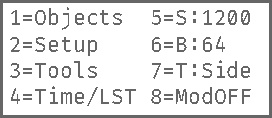
\includegraphics[width=0.8\textwidth]{keypad/AP_menu-1.pdf}
      \caption{main menu}
    \end{figure}
  \column{0.45\textwidth}
  \ \\
    Use \textbf{5=S:1200} from the main menu to set the slew rate.
    
    The slew rate can be set to 600, 900, or 1200 X sidereal rate.
\end{columns}
\end{frame}

% -----------------------------------------------

\begin{frame}[t]{Slewing to Targets}
  \large
  Center  the target in the eyepiece using the \textbf{N/S/E/W} buttons. 
  Once centered, press \textbf{RECAL} and \textbf{NEXT>} simultaneously
  to update the coordinates.
  
\begin{columns}[T]
  \column{0.55\textwidth}
    \begin{figure}[h]
        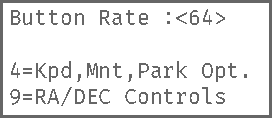
\includegraphics[width=0.8\textwidth]{keypad/AP_menu-shortcut.pdf}
      \caption{quick access}
    \end{figure}
  \column{0.45\textwidth}
  \ \\
    Use \textbf{6=B:64} from the main menu or press \textbf{+/-} to go to the
    quick access menu and use \textbf{\textless PREV/NEXT \textgreater} to change
    the button rate.
\end{columns}
\end{frame}
\subsection{Keypad Database Objects}
% ==============================================

\begin{frame}[t]{\insertsubsectionhead}
  \begin{columns}[T]
  \column{0.55\textwidth}
    \begin{figure}[h]
        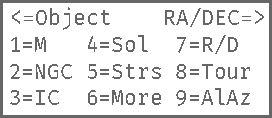
\includegraphics[width=0.8\textwidth]{keypad/AP_menu-objects.pdf}
      \caption{objects menu}
    \end{figure}
  \column{0.45\textwidth}
  % \ \\[0.25ex]
   \textbf{1=Objects} to go to the objects menu.\\[1ex]

    \begin{itemize}
        \item[] \textbf{1=M} (Messier objects)
        \item[] \textbf{2=NGC} (New General Catalog)
        \item[] \textbf{3=IC}   (IC objects from the NGC)
        \item[] \textbf{4=Sol}   (Sun, Moon, and planets)
        \item[] \textbf{5=Strs}  (200 named stars)
    \end{itemize}
\end{columns}
\end{frame}

% -----------------------------------------------

\begin{frame}[t]{Messier \& NGC/IC Objects}
  \begin{columns}[T]
  \column{0.55\textwidth}
    \begin{figure}[ht]
        \begin{subfigure}{0.67\textwidth}
            \frame{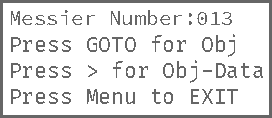
\includegraphics[width=\textwidth]{keypad/AP_menu-objects-1.pdf}}
        \caption{Messier objects}
      \end{subfigure}
      \vspace{\fill}
      \begin{subfigure}{0.67\textwidth}
          \frame{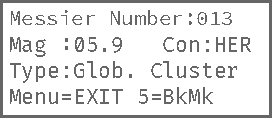
\includegraphics[width=\textwidth]{keypad/AP_menu-objects-1-1.pdf}}
        \caption{object data}
      \end{subfigure}
    \end{figure}
  \column{0.45\textwidth}
  \ \\[0.25ex]
  From the objects menu select \textbf{1=M}, \textbf{2=NGC} or \textbf{3=IC}
  for Messier, NGC, or IC objects.\\[1ex]

  Enter the object ID and press \textbf{GOTO} to slew to the object or
  \textbf{NEXT \textgreater} for object information. \\[1ex]

  From the object data screen select \textbf{5=BkMk} to bookmark for
  later use.
\end{columns}
\end{frame}

% -----------------------------------------------

\begin{frame}[t]{Solar System}
  \begin{columns}[T]
  \column{0.55\textwidth}
    \begin{figure}[ht]
        \begin{subfigure}{0.67\textwidth}
            \frame{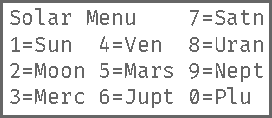
\includegraphics[width=\textwidth]{keypad/AP_menu-objects-4.pdf}}
        \caption{Solar System objects}
      \end{subfigure}
      \vspace{\fill}
      \begin{subfigure}{0.67\textwidth}
          \frame{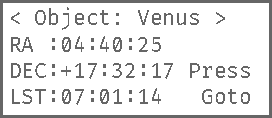
\includegraphics[width=\textwidth]{keypad/AP_menu-objects-4-1.pdf}}
        \caption{object data}
      \end{subfigure}
    \end{figure}
  \column{0.45\textwidth}
  \ \\[0.25ex]
  From the objects menu select \textbf{4=Sol} Solar System objects.\\[1ex]

  Enter \textbf{0--9} for the corresponding object and press \textbf{GOTO} to
  slew to the object or \textbf{\textless PREV/NEXT \textgreater} for object
  information. \\[1ex]
\end{columns}
\end{frame}

% -----------------------------------------------

\begin{frame}[t]{Named Stars}
  \begin{columns}[T]
  \column{0.55\textwidth}
    \begin{figure}[ht]
        \begin{subfigure}{0.67\textwidth}
            \frame{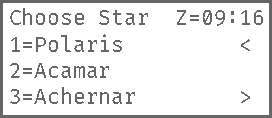
\includegraphics[width=\textwidth]{keypad/AP_menu-objects-5.pdf}}
        \caption{Solar System objects}
      \end{subfigure}
      \vspace{\fill}
      \begin{subfigure}{0.67\textwidth}
          \frame{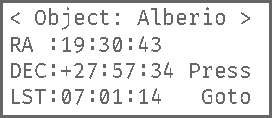
\includegraphics[width=\textwidth]{keypad/AP_menu-objects-5-1.pdf}}
        \caption{object data}
      \end{subfigure}
    \end{figure}
  \column{0.45\textwidth}
  \ \\[0.25ex]
  From the objects menu select \textbf{5=Strs} (200 named stars).\\[1ex]

  Enter \textbf{0--9} for the corresponding star or \textbf{\textless
  PREV/NEXT \textgreater} to scroll through the list. \\[1ex]

  Press \textbf{GOTO} to slew to the star or \textbf{NEXT \textgreater} to
  view the RA and Dec. \\[1ex]

  From the object data screen select \textbf{5=BkMk} to bookmark for later
  use.

\end{columns}
\end{frame}

% -----------------------------------------------

\begin{frame}[t]{Other Stuff}
\begin{columns}[T]
  \column{0.5\textwidth}
  \textbf{6=More}
    \begin{itemize}
    \item Abell Galaxy Clusters
    \item Aitken Double Star Catalog
    \item Palomar Globular Clusters
    \item Uppsalla Galaxy Catalog
    \item Lynds’ Catalog of Bright Nebulae
    \item Lynds’ Catalog of Dark Nebulae
    \item What’s Up Now
    \end{itemize}

  \column{0.5\textwidth}
  \textbf{8=Tour}
    \begin{itemize}
    \item Stars by Constellation
    \item Objects by Constellation
    \item Common Object Names
    \end{itemize}

  \textbf{7=R/D}
    \begin{itemize}
    \item Custom RA \& Dec
    \end{itemize}

  \textbf{9=AlAz}
    \begin{itemize}
    \item Custom Altitude and Azimuth
    \end{itemize}
\end{columns}
\end{frame}

\subsection{Meridian Crossing}
% ==============================================

\begin{frame}[t]{\insertsubsectionhead}
    \begin{columns}[T]
    \column{0.55\textwidth}
      \begin{figure}[ht]
          \begin{subfigure}{0.67\textwidth}
              \frame{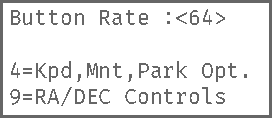
\includegraphics[width=\textwidth]{keypad/AP_menu-shortcut.pdf}}
          \caption{quick-access}
        \end{subfigure}
        \vspace{\fill}
        \begin{subfigure}{0.67\textwidth}
            \frame{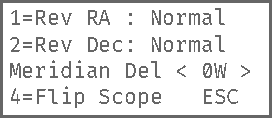
\includegraphics[width=\textwidth]{keypad/AP_menu-ra-dec.pdf}}
          \caption{RA/Dec Controls}
        \end{subfigure}
      \end{figure}
    \column{0.45\textwidth}
    \ \\[0.25ex]
    When the mount limits are set the mount will stop tracking at the
    meridian. \\[1ex]

    You can initiate a meridian flip by executing a \textbf{GOTO} on the object
    again \\[1ex]

    Or from the quick-access menu [ \textbf{+/-}] select \textbf{9=RA/Dec Controls}
    and then \textbf{4=Flip Scope}

  \end{columns}
\end{frame}

% -----------------------------------------------

\begin{frame}[t]{\insertsubsectionhead}
    \begin{columns}[T]
    \column{0.55\textwidth}
      \begin{figure}[ht]
          \begin{subfigure}{0.67\textwidth}
              \frame{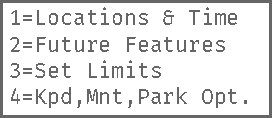
\includegraphics[width=\textwidth]{keypad/AP_menu-setup.pdf}}
          \caption{setup menu}
        \end{subfigure}
        \vspace{\fill}
        \begin{subfigure}{0.67\textwidth}
            \frame{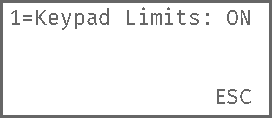
\includegraphics[width=\textwidth]{keypad/AP_menu-setup-3.pdf}}
          \caption{limits}
        \end{subfigure}
      \end{figure}
    \column{0.45\textwidth}
    \textbf{Mount Limits} \\[0.25ex]

    Limits may be toggled on or off by pressing \textbf{2=Setup} and
    then \textbf{3=Set Limits}. \\[1ex]

    It is recommended that you leave the limits set and use the meridian delay
    feature to track past the meridian. 
  \end{columns}
\end{frame}

% -----------------------------------------------

\begin{frame}[t]{\insertsubsectionhead}
    \begin{columns}[T]
    \column{0.55\textwidth}
      \begin{figure}[ht]
          \begin{subfigure}{0.67\textwidth}
              \frame{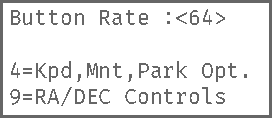
\includegraphics[width=\textwidth]{keypad/AP_menu-shortcut.pdf}}
          \caption{quick-access}
        \end{subfigure}
        \vspace{\fill}
        \begin{subfigure}{0.67\textwidth}
            \frame{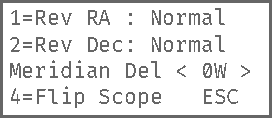
\includegraphics[width=\textwidth]{keypad/AP_menu-ra-dec.pdf}}
          \caption{RA/Dec Controls}
        \end{subfigure}
      \end{figure}
    \column{0.45\textwidth}
    \textbf{Meridian Delay} \\[0.25ex]

    You can use the meridian delay feature to track past the meridian or to
    initiate a meridian flip early. \\[1ex]

    To delay or advance the meridian, from the quick-access menu
    [\textbf{+/-}] select \textbf{9=RA/Dec Controls} and \textbf{\textless
    PREV/NEXT \textgreater} \\[1ex]

    1-6 W will delay 1 to 6 hours, 1-6 E will advance 1 to 6 hours.
  \end{columns}
\end{frame}

% -----------------------------------------------

% \begin{frame}{Problems and Troubleshooting}
%   \Large
%   \begin{itemize}
%     \item[] \textbf{Pointing error}
%     \item[] \textbf{Tracking error}
%     \item[] \textbf{etc.}

% \end{itemize}

% \end{frame}


% ==============================================
\section{References and Documentation}
% ==============================================

\begin{frame}[t]{Observatory Handbook and Manuals}
  \Large
  \begin{itemize}
    \item Printed copies of the telescope and mount manuals are available in the observatory.
    \item PDF versions are also available on the observatory laptop.
    \item There is a Observatory handbook available as a ``work in progress''. Input and
     suggestions would pe appreciated.
    \end{itemize}
\end{frame}

% -----------------------------------------------

\begin{frame}{Observatory Star Charts}
  \begin{columns}[T]
    \column{0.45\textwidth}
    \centering
      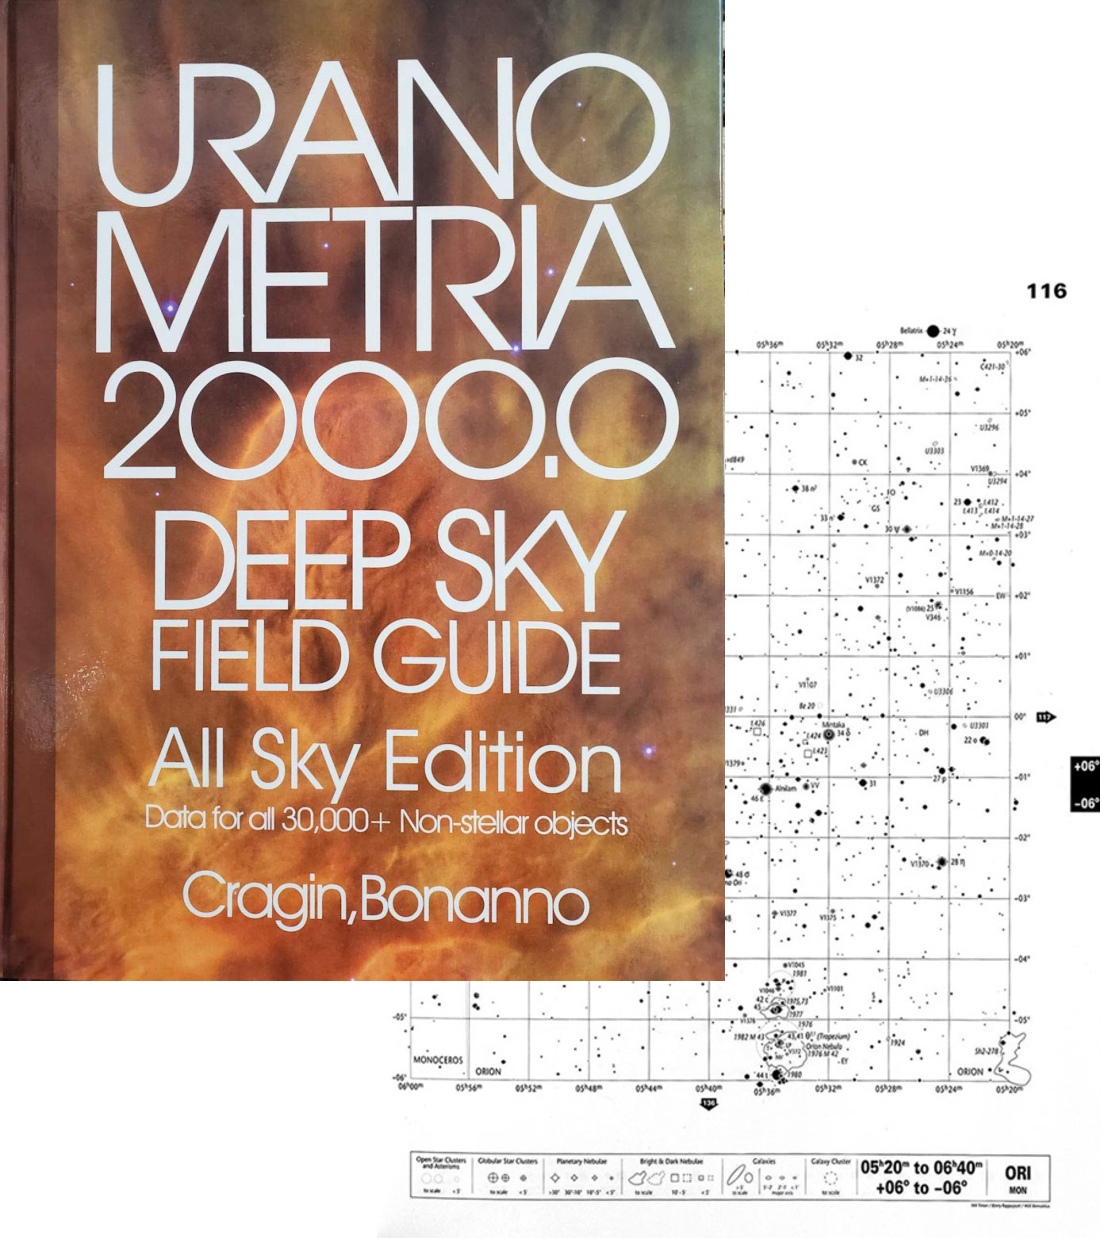
\includegraphics[height=0.8\textheight]{uranometria.pdf}
    \column{0.55\textwidth}
    \ \\[1ex]
    \Large
    \begin{itemize}
      \item 220 charts and 26 close-up charts.
      \item Stars down to mag 9.75.
      \item More than 30,000 non-stellar objects.
      \item Common names, Bayer Stars, Messier, and NGC/IC designations.
      \end{itemize}
  \end{columns}
\end{frame}

% -----------------------------------------------

\begin{frame}{Observatory Star Charts}
  \begin{columns}[T]
    \column{0.45\textwidth}
    \centering
      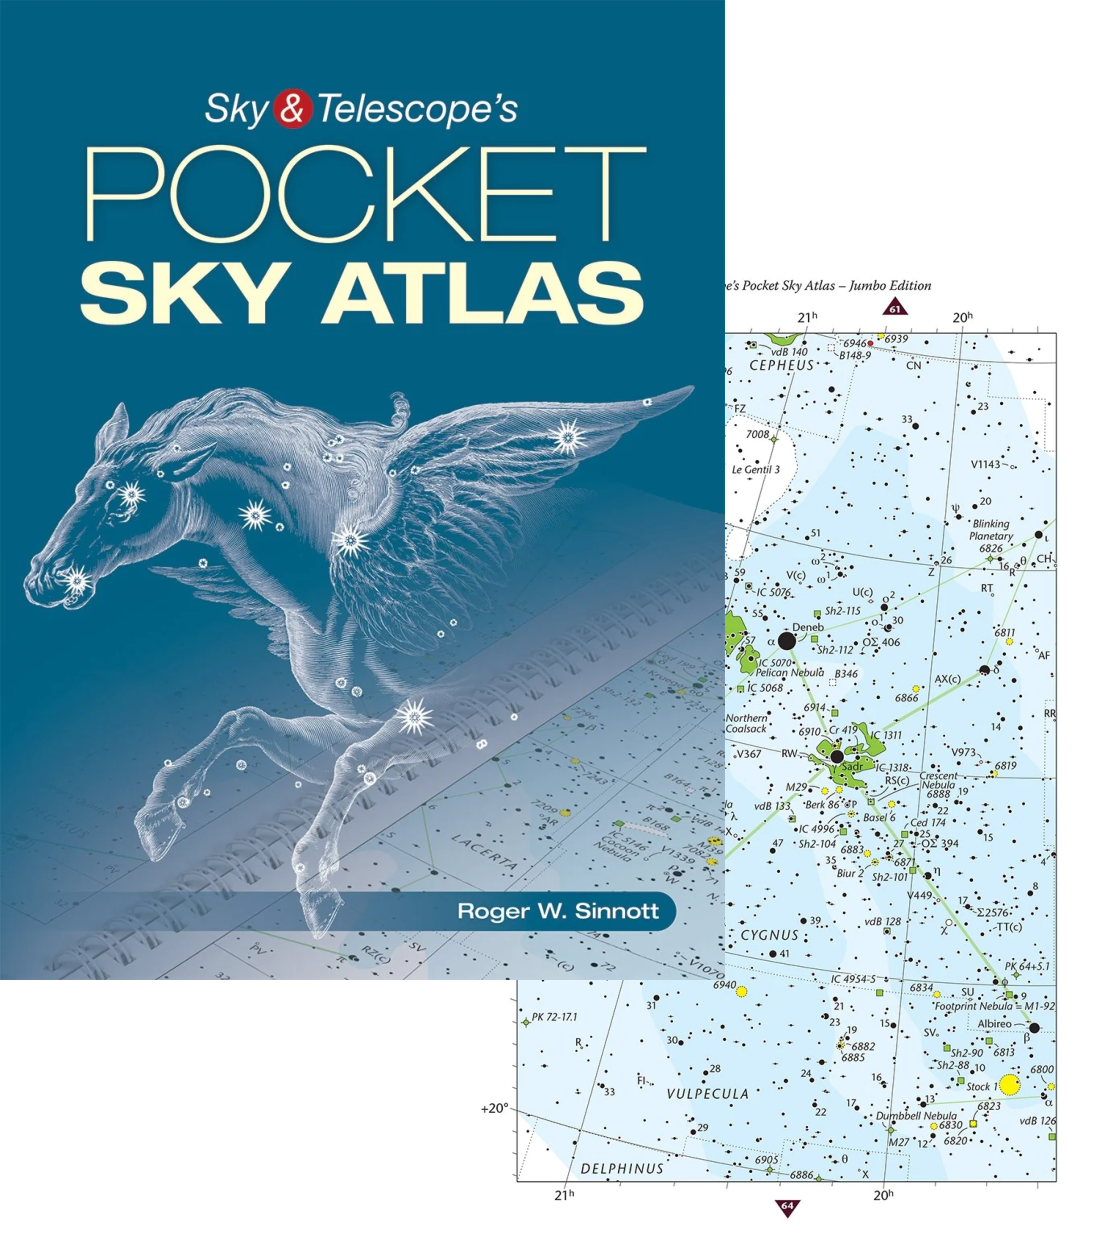
\includegraphics[height=0.8\textheight]{pocket_sky_atlas.pdf}
    \column{0.55\textwidth}
    \ \\[1ex]
    \Large
    \begin{itemize}
      \item 80 charts with 10 close-up charts.
      \item More than 30,000 stars sized according to their relative brightness
      \item 1,500 deep-sky objects color-coded by type.
      \end{itemize}
  \end{columns}
\end{frame}

% -----------------------------------------------

\begin{frame}{Sources}
  Get the source of this presentation from

  \begin{center}
    \small
    \url{https://github.com/Westminster-Astronomical-Society/observatory_handbook}
  \end{center}

  This work is licensed under a
  \href{http://creativecommons.org/licenses/by-sa/4.0/}{Creative Commons
  Attribution-ShareAlike 4.0 International License}.

  \begin{center}\ccbysa\end{center}
\end{frame}


\end{document}
